%! Tex program = xelatex
\documentclass[twoside]{styles/kaobook}
\usepackage{styles/kaorefs}
\usepackage{styles/kao-zh}
\usepackage{styles/kao-ext}

% 用于生成示例文本
\usepackage{lipsum}
\usepackage{zhlipsum} 

\begin{document}
\pagelayout{wide}% Use a wide page layout
\setchapterstyle{plain} % Choose the default chapter heading style
%---------------------------------------------------------------------------------
%	BOOK INFORMATION
%---------------------------------------------------------------------------------

% 设置标题页顶部的内容,允许用户在标题页上方添加自定义内容,如图片、文本等。
\titlehead{\texttt{kaobook}的中文支持和扩展}
% 设置文档的主题或学科,会作为文档标题页上的一部分,展示为“文档主题”。
\subject{Latex的学习系列内容}
% 设置主标题
\title[Example and documentation of the {\normalfont\texttt{kaobook}} class]{{\normalfont\texttt{kaobook}}文档类的中文适配模板}
% 设置副标题
\subtitle{根据您的需要自定义此页面}
% 作者
\author[Federico Marotta]{Tigcat\thanks{一个 \LaTeX 热爱者}}
% 日期
\date{\today}
% 出版社或公司
\publishers{虚拟书社}

\makeatletter
\uppertitleback{\@titlehead} % Header

\lowertitleback{
    \textbf{免责声明}\\
    你可以编辑此页面以满足你的需求。例如,本文中包含了免责声明、书籍说明及其他一些信息。此页面基于~Ken Arroyo Ohori~的论文相应页面和~\href{https://github.com/fmarotta/kaobook/}{kaobook}~宏包作了最小的修改。
 
    \medskip
 
    \textbf{无版权}\\
    \cczero 基于~\href{https://github.com/fmarotta/kaobook/}{kaobook}~宏包的中文翻译和使用已通过~CC0~许可发布至公共领域。在法律允许的范围内,我放弃对此作品的所有版权及相关或邻接权利。
    
    要查看CC0许可协议,请访问:~\\\url{http://creativecommons.org/publicdomain/zero/1.0/}~
    
    \medskip
    
    \textbf{书籍说明} \\
    本文件使用~\href{https://sourceforge.net/projects/koma-script/}{\KOMAScript}~和~\href{https://www.latex-project.org/}{\LaTeX}~的~\href{https://github.com/fmarotta/kaobook/}{kaobook}~宏包进行排版。
    
    本文件的源代码可在以下地址获取:~\\\url{https://github.com/wenhq/template-kaobook-zh}~(欢迎您进行贡献!)
    
    \medskip
    
    \textbf{出版商} \\
    本文件首次发布于2025年2月,由~\@publishers~出版。
}
\makeatother

\maketitle

\frontmatter % START of the pre-document content, uses roman numerals
\chapter*{\centering 序言}
\addcontentsline{toc}{chapter}{序言} % Add the preface to the table of contents as a chapter
LaTeX 就像一座桥梁,将数学与艺术、形式与内容、理性与感性完美融合。它不仅展现了世界的和谐与秩序,还赋予了文字与符号生命,使自然哲学的心灵与灵魂得以深刻表达。在它的帮助下,数学之美被提升到一种诗意的境界,每一个公式、每一行文字,都蕴含着无尽的优雅与智慧,体现了人类对知识与美的追求。

\begin{enumerate}
	\item 这段话是瞎写的;
	\item 这段话是用 GPT-4.1 mini 瞎写的。
\end{enumerate}

LaTeX is like a bridge, perfectly blending mathematics with art, form with content, reason with emotion. It not only showcases the harmony and order of the world but also breathes life into words and symbols, allowing the spirit and soul of natural philosophy to be deeply expressed. With its help, the beauty of mathematics is elevated to a poetic realm, where every formula, every line of text, contains infinite elegance and wisdom, reflecting humanity's pursuit of knowledge and beauty.

\begin{enumerate}
	\item This paragraph is nonsense.
	\item This paragraph is nonsense written using GPT-4.1 mini.
\end{enumerate}

\begin{flushright}
	\textit{Tigcat Wh Q}
\end{flushright}

%----------------------------------------------------------------------------------
%	TABLE OF CONTENTS & LIST OF FIGURES/TABLES
%----------------------------------------------------------------------------------

\begingroup % Local scope for the following commands

% Define the style for the TOC, LOF, and LOT
%\setstretch{1} % Uncomment to modify line spacing in the ToC
%\hypersetup{linkcolor=blue} % Uncomment to set the colour of links in the ToC
\setlength{\textheight}{230\hscale} % Manually adjust the height of the ToC pages

% Turn on compatibility mode for the etoc package
\etocclasstocstyle % "toc display" as if etoc was not loaded
\etocstandardlines % "toc lines" as if etoc was not loaded

\tableofcontents % Output the table of contents

\listoffigures % Output the list of figures

% Comment both of the following lines to have the LOF and the LOT on different pages
\let\cleardoublepage\bigskip
\let\clearpage\bigskip

\listoftables % Output the list of tables

\endgroup


\mainmatter % Denotes the start of the main document content, resets page numbering and uses arabic numbers
\chapter{记录}
在 LaTeX 文档中,\\frontmatter 命令通常用于标记文档的前言部分开始。在 KOMA-Script 文档类(如 scrbook 或 scrreprt)和一些其他文档类中,\\frontmatter 命令之后的内容会使用罗马数字(i, ii, iii, ...)进行页码编号,直到 \\mainmatter 命令,之后的内容会使用阿拉伯数字(1, 2, 3, ...)进行页码编号。

frontmatter 部分通常包括:

封面(Title Page)
版权信息(Copyright Page)
致谢(Acknowledgments)
摘要(Abstract)
目录(Table of Contents)
列表(List of Figures, List of Tables 等)
引言(Introduction)或前言(Preface)
这些部分在书籍和长篇报告中很常见,它们为读者提供了文档的概览和导航。
\setchapterpreamble[u]{\margintoc}
\chapter{主要变动点}
\labch{主要变动点}

\section[原样式修改]{对原始样式的修改}

\href{https://github.com/fmarotta/kaobook}{kaobook 项目}通过提供一系列 LaTeX 文档类和宏包,为学术著作和技术文档的排版提供了强大的支持。

Kaobook模板相关文件包括 kaobook.cls、kao.sty、kaobiblio.sty、kaorefs.sty 和 kaotheorems.sty,这些文件可以灵活的引用。它们的主要作用为:

\begin{itemize}
    \item \textbf{kaobook.cls‌} 作为主文档类文件定义了文档的整体排版框架,包括页边距、章节样式、多级标题等。它支持分页控制、多语言兼容等书籍排版特性,为文档提供统一且专业的外观。
    \item \textbf{kao.sty} 基础样式包提供了颜色方案、自定义命令和工具函数等底层支持。这些功能被广泛应用于文档中的代码高亮、侧边注释等场景,是其他扩展样式包的基础依赖。
    \item \textbf{kaobiblio.sty} 是参考文献处理模块, 集成并扩展了 biblatex 的功能,预设了符合 kaobook 风格的引用格式(如作者-年份或数字标号)。它支持多文献库管理,简化了参考文献的插入和格式化过程。
    \item \textbf{kaorefs.sty} 交叉引用增强工具优化了图表、章节等元素的智能引用显示。它支持超链接跳转和动态标签生成,提高了文档中交叉引用的可读性和易用性。
    \item 数学环境定制包,\textbf{kaotheorems.sty} 提供了统一风格的定理、引理、证明等数学环境框。这些框支持可折叠功能,便于读者浏览和隐藏数学证明等细节内容。同时,它还支持自定义编号规则和边注标记,满足了复杂数学文档的排版需求。
\end{itemize}

本项目引入了 kaobook.cls、kao.sty和kaorefs.sty三个文件。在引入原始 .cls 或 .sty 文件时,尽量避免修改原文件内容,以便在原项目升级时能够方便地进行集成。尽管如此,仍然不可避免地会遇到一些不适应中文排版的警告或错误,需要针对这些问题进行修复和调整。


\subsection{kaobook.cls‌的变动}
由于要引入 styles 文件夹下的对应文件,因此在第28行,将 \mintinline{latex}|\ProvidesClass{kaobook}| 改为 \mintinline{latex}|\ProvidesClass{styles/kaobook}|;在第44行,将 \mintinline{latex}|\RequirePackage{kao}| 改为 \mintinline{latex}|\RequirePackage{styles/kao}|。

另外,因为中文无法支持“小型大写字母”这样的字体,为避免编译告警故删除了第254和255行的 \mintinline{latex}|\scshape| 命令,如~\reflistings{kaobookcls删除scshape命令}~所示。

\begin{listing}[H]
    \begin{minted}[linenos=false]{latex}
        \addtokomafont{part}{\normalfont\bfseries}
        \addtokomafont{partentry}{\normalfont\bfseries}
    \end{minted}
    \caption{删除 scshape 后的 kaobook.cls‌ 文件}
    \lablistings{kaobookcls删除scshape命令}
\end{listing}

\subsection{kao.sty的变动}
kao.sty文件同样要指定到 styles 文件夹下,修改文件第1行为 \mintinline{latex}|\ProvidesPackage{styles/kao}|。

一些兼容性的修改,如第19行删除了 usenames,改为 \newline \mintinline{latex}|\RequirePackage[dvipsnames,table]{xcolor}|; \newline 第29行增加了 listings=false, 改为 \newline \mintinline{latex}|\AtEndPreamble{\RequirePackage[listings=false]{scrhack}}|; 第240行增加了 singlespacing=true,改为 \newline \mintinline{latex}|\RequirePackage[singlespacing=true]{scrlayer-scrpage}|。

调整了目录的深度,从 section 调整到 subsection,文件第1208行改为 \mintinline{latex}|bookmarksdepth=subsection,|。

\subsection{kaorefs.sty的变动}
kaorefs.sty文件类似地修改到 styles 文件夹下,修改文件第1行为 \mintinline{latex}|\ProvidesPackage{styles/kaorefs}|。

注释掉第41行,以及从48行到148行这段多语言支持的部分。

\section[kao-zh.sty中文支持]{新增kao-zh.sty中文支持文件}

新增的 kao-zh.sty 宏包文件是通过 ctex 包来支持中文的显示,并且通过这个文件对 kaobook 中的关键字展示采用中文重定义,并规定了文档的字体。

\subsection{ctex宏包}

在 kao-zh.sty 文件中引入 ctex 宏包来支持中文,引用时不指定具体字体,后续使用自定义的开源字体代替。

在 \reflistings{kao-zh.sty中引入ctex宏包} 里,如果不准备自定义字体,可以将fontset=none改为对应的mac或windows。

\begin{listing}[H]
    \begin{minted}[linenos=false]{latex}
        \RequirePackage[UTF8, fontset=none, scheme=chinese]{ctex}
    \end{minted}
    \caption{kao-zh.sty中引入ctex宏包}
    \lablistings{kao-zh.sty中引入ctex宏包}
\end{listing}

ctex 是一个专门为支持中文排版而设计的 LaTeX 宏包\sidenote{关于 ctex 宏包的详细文档,可以参考\href{https://www.ctan.org/pkg/ctex}{CTeX 官方文档}},它是LaTeX 中是中文排版里最常用的标准方案,为 LaTeX 提供了对中文字符、字体、段落、编码等的良好支持。

\subsection{标题文本的中文重定义}
对于 kao 样式里定义的一些标题文本,在本项目中进行了重新定义\sidenote{在英文环境中更改特定标签(如目录、插图、表格等)的名称,\textbf{应该有更好的修改方式}。}。如 \reflistings{kao-zh.sty中的标题文本重定义} 里的重新定义命令,可以修改以适配自己需要的中文。

\begin{listing}[H]
    \begin{minted}[linenos=false]{latex}
        \RequirePackage[english]{babel}
        \renewcaptionname{english}{\contentsname}{目录}
        \renewcaptionname{english}{\listfigurename}{插图}
        \renewcaptionname{english}{\listtablename}{表格}
        \renewcaptionname{english}{\indexname}{索引}
        \renewcaptionname{english}{\bibname}{参考文献}
        \renewcaptionname{english}{\figurename}{图}
        \renewcaptionname{english}{\tablename}{表}
        
        \renewcommand{\lstlistlistingname}{代码列表}
    \end{minted}
    \caption{kao-zh.sty中的标题文本重定义}
    \lablistings{kao-zh.sty中的标题文本重定义}
\end{listing}

\subsection{自定义字体}
为了避免使用系统默认字体可能带了的商业使用法律问题,本项目采用了开源免费商用字体。这部分内容可以根据需要自行修改。

\subsubsection{中文字体}

本项目采用 \href{https://github.com/takushun-wu/WenYuanFonts}{WenYuanFonts 项目}提供的文源字体\sidenote{基于思源字体二次开发,开源免费商用。}作为文档字体,另采用 \href{https://github.com/subframe7536/maple-font}{maple-font 项目}提供的Maple Mono 字体\sidenote{开源等宽字体,中英文宽度完美 2:1。}作为文档的等宽字体。所有使用到的字体文件参考 \nrefsec{代码目录结构} 的内容都放在了 font 目录下,且注意,\textbf{字体文件不保证为最新}。

\begin{listing}[H]
    \begin{minted}[linenos=false]{latex}
        \setCJKmainfont [Path={font/}, AutoFakeBold, AutoFakeSlant] {WenYuanMincho-Regular.ttf}
        % 中文无衬线字体
        \setCJKsansfont [Path={font/}, BoldFont={WenYuanGothic-Medium.ttf}, AutoFakeSlant] {WenYuanGothic-Regular.ttf}
        % 中文等宽字体
        \setCJKmonofont [Path={font/}, BoldFont={MapleMonoNormalNL-NF-CN-Bold.ttf},  ItalicFont={MapleMonoNormalNL-NF-CN-Italic.ttf}] {MapleMonoNormalNL-NF-CN-Light.ttf}
    \end{minted}
    \caption{kao-zh.sty中使用的中文字体}
    \lablistings{kao-zh.sty中使用的中文字体}
\end{listing}

如 \reflistings{kao-zh.sty中使用的中文字体} 所示\sidenote{有些地方配置了 AutoFakeBold 和 AutoFakeSlant,没有什么原因,只是懒得去下载字体了。},中文有衬线字体使用文源宋体(WenYuanMincho)、中文无衬线字体使用文源黑体(WenYuanGothic)、等宽字体使用 Maple Mono 字体。

\subsubsection{英文字体}

当前使用了 TeX Gyre 系列的字体,准备改为 Times 字体。\todo{使用Times New Roman字体的正确姿势} 

\iffalse
\section{后续内容}
\subsection{富强民主}
\zhlipsum[3]
\fi
\setchapterpreamble[u]{\margintoc}
\chapter{使用 kaobook 的姿势}
\labch{使用 kaobook 的姿势}

\todo[inline]{使用 kaobook 的姿势}

\section{插入图片}

\section{插入表格}

\section{使用注释}

\section{使用提示框}


\section{其他}


\setchapterstyle{bar}
\pagelayout{wide} % No margins
\addpart{附\ 录}
\appendix
\chapter{字体相关}

字体的使用是 \LaTeX 里绕不过去的话题,本篇附录用于记录字体使用的一些内容。

\section{Times New Roman字体}
\labsec{Times New Roman字体}
本文来源 \href{https://www.latexstudio.net/archives/9323.html}{LaTeX技巧885:LaTeX下使用Times New Roman字体的正确姿势},引用为附录内容进行了简化和修改。

Times New Roman 字体由 Monotype 公司于1932年发表,并为英国的《泰晤士报》首次采用。这是一个经典的、中规中矩的字体,所以经常被选为西文的标准字体之一。

\begin{itemize}
    \item Windows 中使用的 Times New Roman 是 Monotype 在最初字形上稍加修改(字宽方面)得到的。
    \item macOS 系统中使用的 Times Roman 是 Linotype 公司出品的,它与 Monotype 家的 Times New Roman 除了个别字形稍有区别之外(相信你看不出来),几乎完全相同。
    \item 开源系统中对应的字体,则是 URW 的 Nimbus Roman No9 L 字体,它在 GPL 许可下发布。
\end{itemize}

它们几乎没有差别。

最推荐的方法是使用 fontspec 系列宏包,直接选取系统中的字体,如~\reflistings{引用 ontspec宏包使用Times New Roman字体}~所示。。

\begin{listing}[H]
    \begin{minted}[]{latex}
        \documentclass{article}
        \usepackage{fontspec}
        \setmainfont{Times New Roman}
        \usepackage{mathspec}
        \setmathfont{Times New Roman}
        \begin{document}
        This is the typeface Times New Roman.
        
        Enjoy!
        \end{document}
    \end{minted}
    \caption{引用 fontspec 宏包使用 Times New Roman 字体}
    \lablistings{引用 ontspec宏包使用Times New Roman字体}
\end{listing}
\chapter{画图 tikz}

\section{使用代码嵌入还是文件嵌入}

在 \LaTeX 中使用 TikZ 绘图有两种主要方式:直接嵌入代码和外部生成后嵌入。两种方法各有优缺点。

\subsection{比较}

先说结论:两种方式都能保留矢量效果;外部生成后嵌入的方式编译速度明显更快。

实践建议:简单图形 - 直接嵌入LaTeX文档;复杂图形 - 使用externalize功能;超复杂图形 - 考虑完全外部化,使用单独的文件生成后导入;需要频繁修改调试的图形 - 先在单独文件中开发和测试,完成后再整合到文档中。

\subsubsection{直接嵌入TikZ代码}

\paragraph{优点}

\begin{itemize}
    \item 保留完整矢量图质量,缩放不失真
    \item 图形字体与文档保持一致性
    \item 便于随时修改图形
    \item 可引用文档中的变量和参数
    \item 与文档完全集成,便于版本控制
\end{itemize}

\paragraph{缺点}

\begin{itemize}
    \item 编译速度较慢,每次都需重新生成图形
    \item 复杂图形会消耗大量内存
    \item 调试可能较为困难
\end{itemize}

\subsubsection{外部生成PDF后嵌入}

\paragraph{优点}

\begin{itemize}
    \item 编译速度快,图形只需生成一次
    \item 降低主文档复杂度
    \item 图形可在多个文档中重用
    \item 可单独调试图形
\end{itemize}

\paragraph{缺点}

\begin{itemize}
    \item 工作流程较复杂,需维护额外文件
    \item 修改图形需重新编译外部文件
    \item 无法直接引用主文档中的变量
\end{itemize}

\subsection{最佳实践:TikZ外部化功能}

可使用 \mintinline{latex}{externalize} 库结合两种方法的优点:

\begin{listing}[H]
    \begin{minted}{latex}
        \usepackage{tikz}
        \usetikzlibrary{external}
        \tikzexternalize[prefix=tikz/]
    \end{minted}
    \caption{导言区external宏包以及配置}
    \lablistings{导言区external宏包以及配置}
\end{listing}

\begin{figure}[htbp]
    \centering
    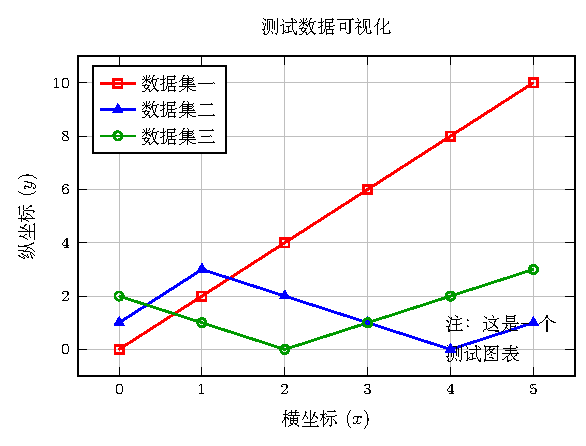
\includegraphics[width=0.6\textwidth]{plots/plot_test.pdf}
    \caption{这是一个通过独立编译生成的测试数据可视化图表。}
    %\label{fig:my_plot} % 为图表设置一个标签,方便交叉引用
\end{figure}

\backmatter
%----------------------------------------------------------------------------------
%	ACKNOWLEDGMENTS PAGE
%----------------------------------------------------------------------------------
\chapter*{\centering 致谢} \todo{致谢部分待补充}
\addcontentsline{toc}{chapter}{致谢} % 将致谢添加到目录中

本文源于2024年从~\href{https://www.latexstudio.net/}{\LaTeX 工作室} 看到了有关 ~\\\url{https://github.com/JimRou/template_kaobook} 的介绍。

\end{document}

